
%(BEGIN_QUESTION)
% Copyright 2006, Tony R. Kuphaldt, released under the Creative Commons Attribution License (v 1.0)
% This means you may do almost anything with this work of mine, so long as you give me proper credit

When using load cells to measure vessel level, certain precautions must be taken to ensure accurate measurements:

$$\includegraphics[width=15.5cm]{i00326x01.eps}$$

One important precaution to take is installing flexible couplings on all pipes leading into and out of the vessel.  Rigid pipes will cause measurement errors -- explain why this is.

\vskip 10pt

Supposing this (vertical) cylindrical storage tank is 10 feet in diameter, 8 feet high from the tank bottom to the base of the conical roof (11 feet from the tank bottom to the roof peak), fabricated entirely of mild steel, and weighs 12,933 pounds when empty, calculate the liquid level inside the tank at a measured total weight of 40,854 pounds.  Assume a liquid with a density of 60.5 pounds per cubic foot.

\vskip 20pt \vbox{\hrule \hbox{\strut \vrule{} {\bf Suggestions for Socratic discussion} \vrule} \hrule}

\begin{itemize}
\item{} Identify some practical applications in industry where weight-based level measurement would be preferable over other technologies.
\item{} One of the factors potentially causing measurement errors in a system such as this {\it weather}, at last for vessels located outside.  Identify some specific weather conditions that could cause problems, and explain how those problems would show up in the vessel's level indication signal.
\end{itemize}

\underbar{file i00326}
%(END_QUESTION)





%(BEGIN_ANSWER)

Liquid level = 5 feet 10.5 inches from bottom of tank

%(END_ANSWER)





%(BEGIN_NOTES)

External piping cannot be allowed to bear any of the vessel's weight.

\vskip 10pt

Total weight $-$ tare weight = product weight

\vskip 10pt

40854 lb $-$ 12933 lb = 27921 lb

$$F = \gamma V$$

$$V = {F \over \gamma} = {27921 \hbox{ lb} \over 60.5 \hbox{ lb/ft}^3} = 461.5 \hbox{ ft}^3$$

$$V = Ah$$

$$h = {V \over A}$$

$$A = \pi r^2 = \pi 5^2 = 78.54 \hbox{ ft}^2$$

$$h = {V \over A} = {461.5 \hbox{ ft}^3 \over 78.54 \hbox{ ft}^2} = 5.876 \hbox{ ft} = 5 \hbox{ ft } 10.5 \hbox{ in}$$

\vskip 10pt

The tank's material (mild steel) is extraneous information, included for the purpose of challenging students to identify whether or not information is relevant to solving a particular problem.

%INDEX% Measurement, level: load cell

%(END_NOTES)


